\subsection{Base-Policy Skill Learning and Retention}\label{sec:skill_retention}
These measurements concern dense-reward training of simple CDPR skills and their consolidation into a base policy (S1--S4), before full-task composition. Each skill uses the instruction and reset protocol in Section~\ref{sec:skill_acquisition}; placement tests start with the object already held. Learning a new skill can degrade previously learned behavior, which full-task execution later needs.

In a forgetting evaluation, mean reaching success falls from 64.1\% for the reaching reference to 5.3\% after placement RL, over three evaluation rounds per condition. The recovery evaluation in Fig.~\ref{fig:retention} is a separate measurement: balanced self-imitation raises reaching success from 8.0\% to 31.1\%. Plate placement changes from 50.0\% to 52.3\%, and bowl placement from 23.05\% to 27.65\%. The bank combines earlier reaching successes with current placement successes, balancing the retained data by instruction.

\begin{figure}[!t]
\centering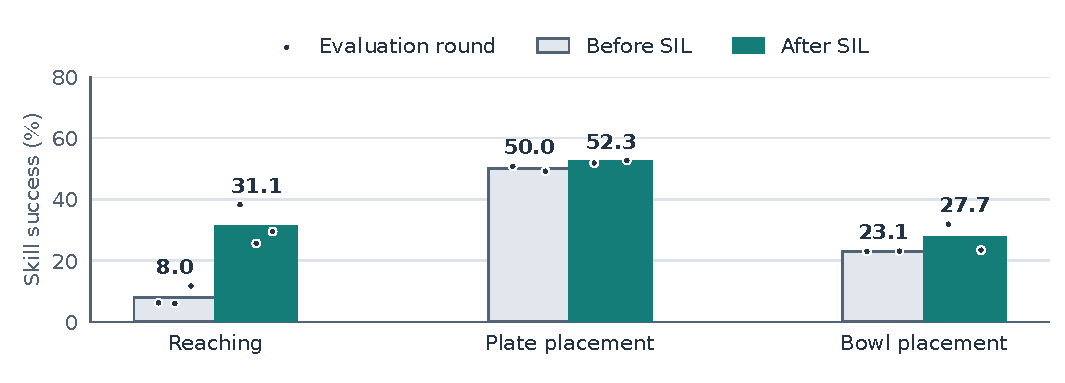
\includegraphics[width=\columnwidth]{figures/skill_retention.pdf}
\caption{Base-policy skill recovery before full-task composition. Bars show means and points show individual evaluation rounds: three for reaching and two for each placement skill, per condition. Reaching uses the instruction \emph{move to \textless object\textgreater}; placement starts with the object already held. Reaching partially recovers while both placement means increase.}
\label{fig:retention}
\end{figure}

Recovery is partial, with placement performance retained while reaching improves. These measurements cover approach and placement. They do not isolate the contribution of self-imitation to final full-task success, and no unbalanced-replay control was run.
